
\section{Versuchsaufbau und Durchführung}
\label{sec:Durchführung}
\subsection{Vorbereitungsaufgaben}
\label{subsec:Aufgaben}
Zur Vorbereitung auf den Versusch sollten die Dichte $\rho$, die spezifische Wärme $c$ und
die Wärmeleitfähigkeit $\kappa$ von Aluminium, Edelstahl, Messing und Wasser recherchiert werden.\\
Diese sind in \autoref{tab:Tabelle1} aufgeführt.
\begin{table}[H]
    \centering
    \caption{Alle hier aufgeführten Literaturwerte sind bei Raumtemperatur(20$\unit{\celsius}$) genommen. \\Quellen:\cite{stahl};\cite{demt};\cite{Geschke}; }
    \label{tab:Tabelle1}
    \begin{tabular}{cccc}
        \toprule
        Stoff&
        {$c \left[\frac{\symup{J}}{\symup{gK}}\right]$} &
        {$\rho \left[\frac{\symup{kg}}{\symup{m}^3}\right]$} &
        {$\kappa \left[\frac{\symup{W}}{\symup{mK}}\right]$} \\
        \midrule
        Aluminium & 0.896 & 2700 & 237.0 \\
        Edelstahl & 0.500 & 7900 & 113.0 \\
        Messing(CuZn37) & 0.380 & 8400 & 15.0 \\
        Wasser & 4.182 & 998 & 0.6 \\
        \bottomrule
    \end{tabular}
\end{table}
\subsection{Aufbau}
\label{subsec:Aufbau}
Für den Versuch wird eine Platine mit vier Probestäben (2 x Messing, 1 x Aluminium und 1 x Edelstahl)
verwendet, wie sie in \autoref{fig:Plat} zu sehen ist. \\
Darauf sind die Thermoelemente T1-T8, jeweils zwei
an zwei verschiedenen Stellen je Stab, und in der Mitte das Peltier-Element zum Erhitzen der Stäbe installiert.\\
Dies wird mit dem Schalter rechts oben auf der Platine ein- und ausgeschaltet. \\
Alle gemessenen Temperaturen der Thermoelemente werden an ein 8-faches Temperaturarray
übermittelt und von jenem zum Datenlogger 'Xplorer GLX'(siehe \autoref{fig:GLX}) zwecks Erfassung weitergeleitet. \\
Die Probestäbe haben die in \autoref{fig:Masse} angegebenen Maße und Materialeigenschaften.
\begin{figure}[H]
    \centering
    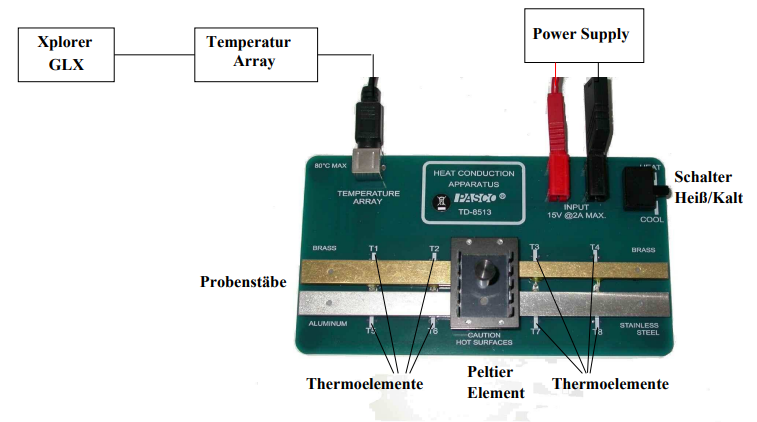
\includegraphics[scale=0.8]{content/Aufbau.png}
    \caption{Die im Experiment verwendete Versuchsplatine mit Beschriftung der Elemente darauf, sowie der angeschlossenen Geräte. \\Quelle:\cite{sample}}
    \label{fig:Plat}
\end{figure}
\begin{figure}[H]
    \centering
    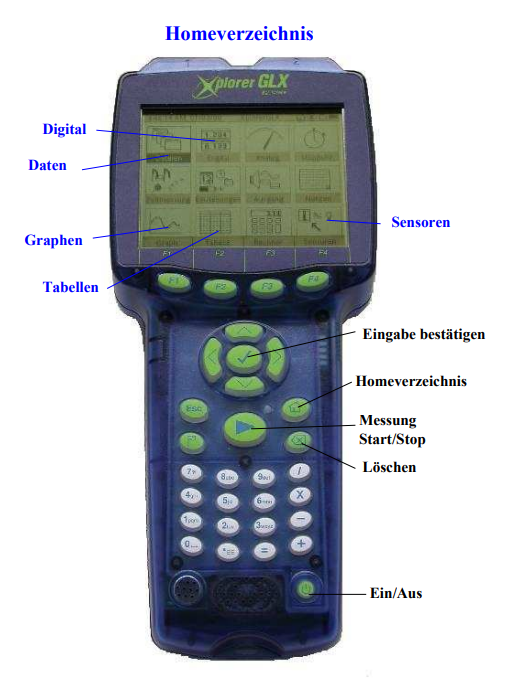
\includegraphics[scale=0.6]{content/GLX.png}
    \caption{Eine Abbildung des Xplorer GLX mitsamt der Tastenbeschriftung. Quelle:\cite{sample}}
    \label{fig:GLX}
\end{figure}
\begin{figure}[H]
    \centering
    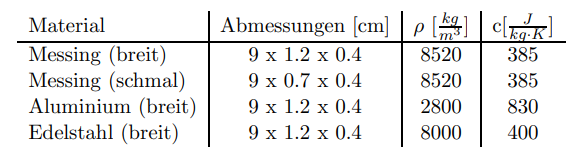
\includegraphics[scale=1]{content/StabDaten.png}
    \caption{Die Tabelle mit den Maßen und Materialeigenschaften der Probestäbe. Quelle:\cite{sample}}
    \label{fig:Masse}
\end{figure}
\subsection{Aufgaben und Durchführung}
\label{subsec:AufgDurch}
Es soll für alle vier Stäbe der gemessene zeitliche Verlauf der Temperaturänderung mit der statischen und
der dynamischen Methode untersucht werden. \\
Zudem sollen die Wellenlänge, die Frequenz der Temperaturwelle
nach periodischer Anregung und außerdem die Wärmeleitfähigkeit der drei Materialien nach
der Angström-Methode (dynamische Methode) bestimmt werden.
\subsubsection{Durchführung statische Methode}
Für die statische Messung wurde am Datenlogger die Abtastrate $\symup{\Delta}t_{GLX}$ auf $\SI{5}{\second}$ und die Spannung
$U_P$ am Power Supply auf $\SI{5}{\volt}$ eingestellt. Außerdem ist der Datenlogger so eingerichtet worden, dass alle acht Sensoren
erfasst werden. \\
Es werden vor dem Start jeder Messung die Wärmeisolierungen auf die Stäbe gelegt, um den Wärmeverlust zu verringern.\\
Sie werden nach Abschluss der jeweiligen Messung abgenommen und das Peltier-Element auf 'COOL' eingestellt, sodass die Stäbe abkühlen.\\
Bei dieser Messreihe ist nach dem Einstellen des Peltier-Elementes auf 'HEAT' solange gemessen worden, bis ein Thermoelement, in diesem Falle
Thermoelement T7, ca. $\SI{45}{\celsius}$ erreicht hatte. \\
Nach Abschluss der Messreihe wurden die Stäbe an der Luft
auf unter $\SI{30}{\celsius}$ gekühlt und die Daten dem Datenlogger mit einem USB-Stick entnommen.
\subsubsection{Durchführung dynamische Methode}
Bei der dynamischen Methode, auch Angström-Methode genannt, werden die Stäbe periodisch erwärmt.\\
Am Datenlogger wurde hierbei die Abtastrate $\symup{\Delta}t_{GLX}$ auf $\SI{2}{\second}$
und die Spannung $U_P$ am Power Supply auf $\SI{8}{\volt}$ eingestellt.\\ 
Die erste Messreihe
wurde mit einer Periodendauer von $\SI{80}{\second}$, also für $\SI{40}{\second}$ der Schalter auf 'HEAT' und dann
$\SI{40}{\second}$ auf 'COOL' eingestellt. \\
Es wurde die Messreihe nach dem Messen von 10 Perioden beendet und die Stäbe abgekühlt.\\
In der zweiten Messreihe ist nahezu genauso verfahren worden, wie in der ersten Messreihe der dynamischen Methode. \\
Als Periodendauer wurden hier
$\SI{200}{\second}$ verwendet und die Messung beendet, als eines der Thermoelemente $\SI{80}{\celsius}$ erreicht hat.\\
Anschließend wurden die Stäbe wieder gekühlt.
\subsubsection{Abstände der Thermoelemente}
Zuletzt sind die Abstände $\symup{\Delta}x$ der Thermoelemente an jedem Stab mit einer Schieblehre gemessen worden.\\